% ==============================================================================
%                                    DVG303
%                  Objektorienterad Design och Programmering
%                                Laboration #1
%
% Author:   Jonas Sjöberg
%           Högskolan i Gävle
%           tel12jsg@student.hig.se
%           https://github.com/jonasjberg
%
% License:  Creative Commons Attribution-NonCommercial-ShareAlike 4.0
%           International.  See LICENSE.md for full licensing information.
% ==============================================================================

\renewcommand{\thesubsection}{(\alph{subsection})}

\section{Uppgift 2}\label{sec:uppg2}

\subsection{}\label{sec:uppg2a}
\subsubsection*{Frågeställning}
En superklass kan innehålla attribut och operationer som är gemensamma
för ett antal klasser.  Beskriv en superklass till klasserna ni skapade i
uppgift 1! Beskrivningen ska innehålla information om vilka attribut det ska
finnas i superklassen och vilka meddelanden (kommandon och frågor) man kan
skicka till instanser av superklasstypen.  Förklara varför ni bestämde er
för just den uppsättning attribut/operationer som ni valde!


\subsubsection*{Lösning}
Figurerna beskrivs av ett visst antal punkter eller positioner som representeras
av \texttt{Vertex2D}-instanser. Alla figurer består av minst ett
\texttt{Vertex2D}-objekt som representerar figurens mittpunkt. Figurerna kan
delas upp i två separata grenar i arvshierarkin, \texttt{Figure} och
\texttt{SimpleFigure}.  Skillnaden mellan Figure och SimpleFigure är hur många
punkter de lagrar för att beskriva figuren de representerar.  Figurer som kan
beskrivas med bara en \texttt{Vertex2D}-instans, figurens position, ärver från
\texttt{SimpleFigure}; punkt, cirkel och ellips.  Figurer som består av fler
\texttt{Vertex2D}-objekt, ärver från \texttt{Figure}.  Klassen \texttt{Figure}
lagrar sina punkter i en lista för enkel åtkomst.  Det möjliggör också
skapandet av figurer med ett godtyckligt antal punkter.


\subsection{}\label{sec:uppg2b}
\subsubsection*{Frågeställning}
Ska superklassen vara en abstrakt klass eller inte? Diskutera vad som talar
emot och vad som talar för!

\subsubsection*{Lösning}
Klasserna \texttt{SimpleFigure} och \texttt{Figure} är både abstrakta av den
anledningen att vi sannolikt inte kommer att behöva instantiera någon odefinerad
figur. Möjligheten att skapa t.ex. en polygon med ett godtyckligt antal punkter
från figurklasserna talar emot att de är abstrakta, det skulle vara möjligt att
skapa odefinerade figur-objekt och efter att de skapats namnge dem till
rätt figur (punkt, kvadrat, triangel, etc..) efter det antal punkter figuren
instantierats med och dessa punkters position.
I det här fallet valde jag ändå att göra figurklasserna abstrakta och låta
subklasserna punkt, kvadrat, triangel, etc.. ärva från superklasserna och
utgöra faktiska, instantierbara objekt.
De olika figurerna har fält och metoder som gör dem unika, en cirkel har t.ex.
en radie medan en ellips har en bredd och höjd.


\subsection{}\label{sec:uppg2c}
\subsubsection*{Frågeställning}
Uppdatera klassdiagrammet från uppgift 1, så att den nya klassen ingår i
modellen samt relationerna mellan superklassen och befintliga klasser!

\subsubsection*{Lösning}
\par UML-klassdiagrammet och arvshierarkin återfinns i Figur~\ref{fig:uppg2a},
 samt bifogad fil.

%\begin{figure}[htbp]
\begin{sidewaysfigure}[ht]
\centering
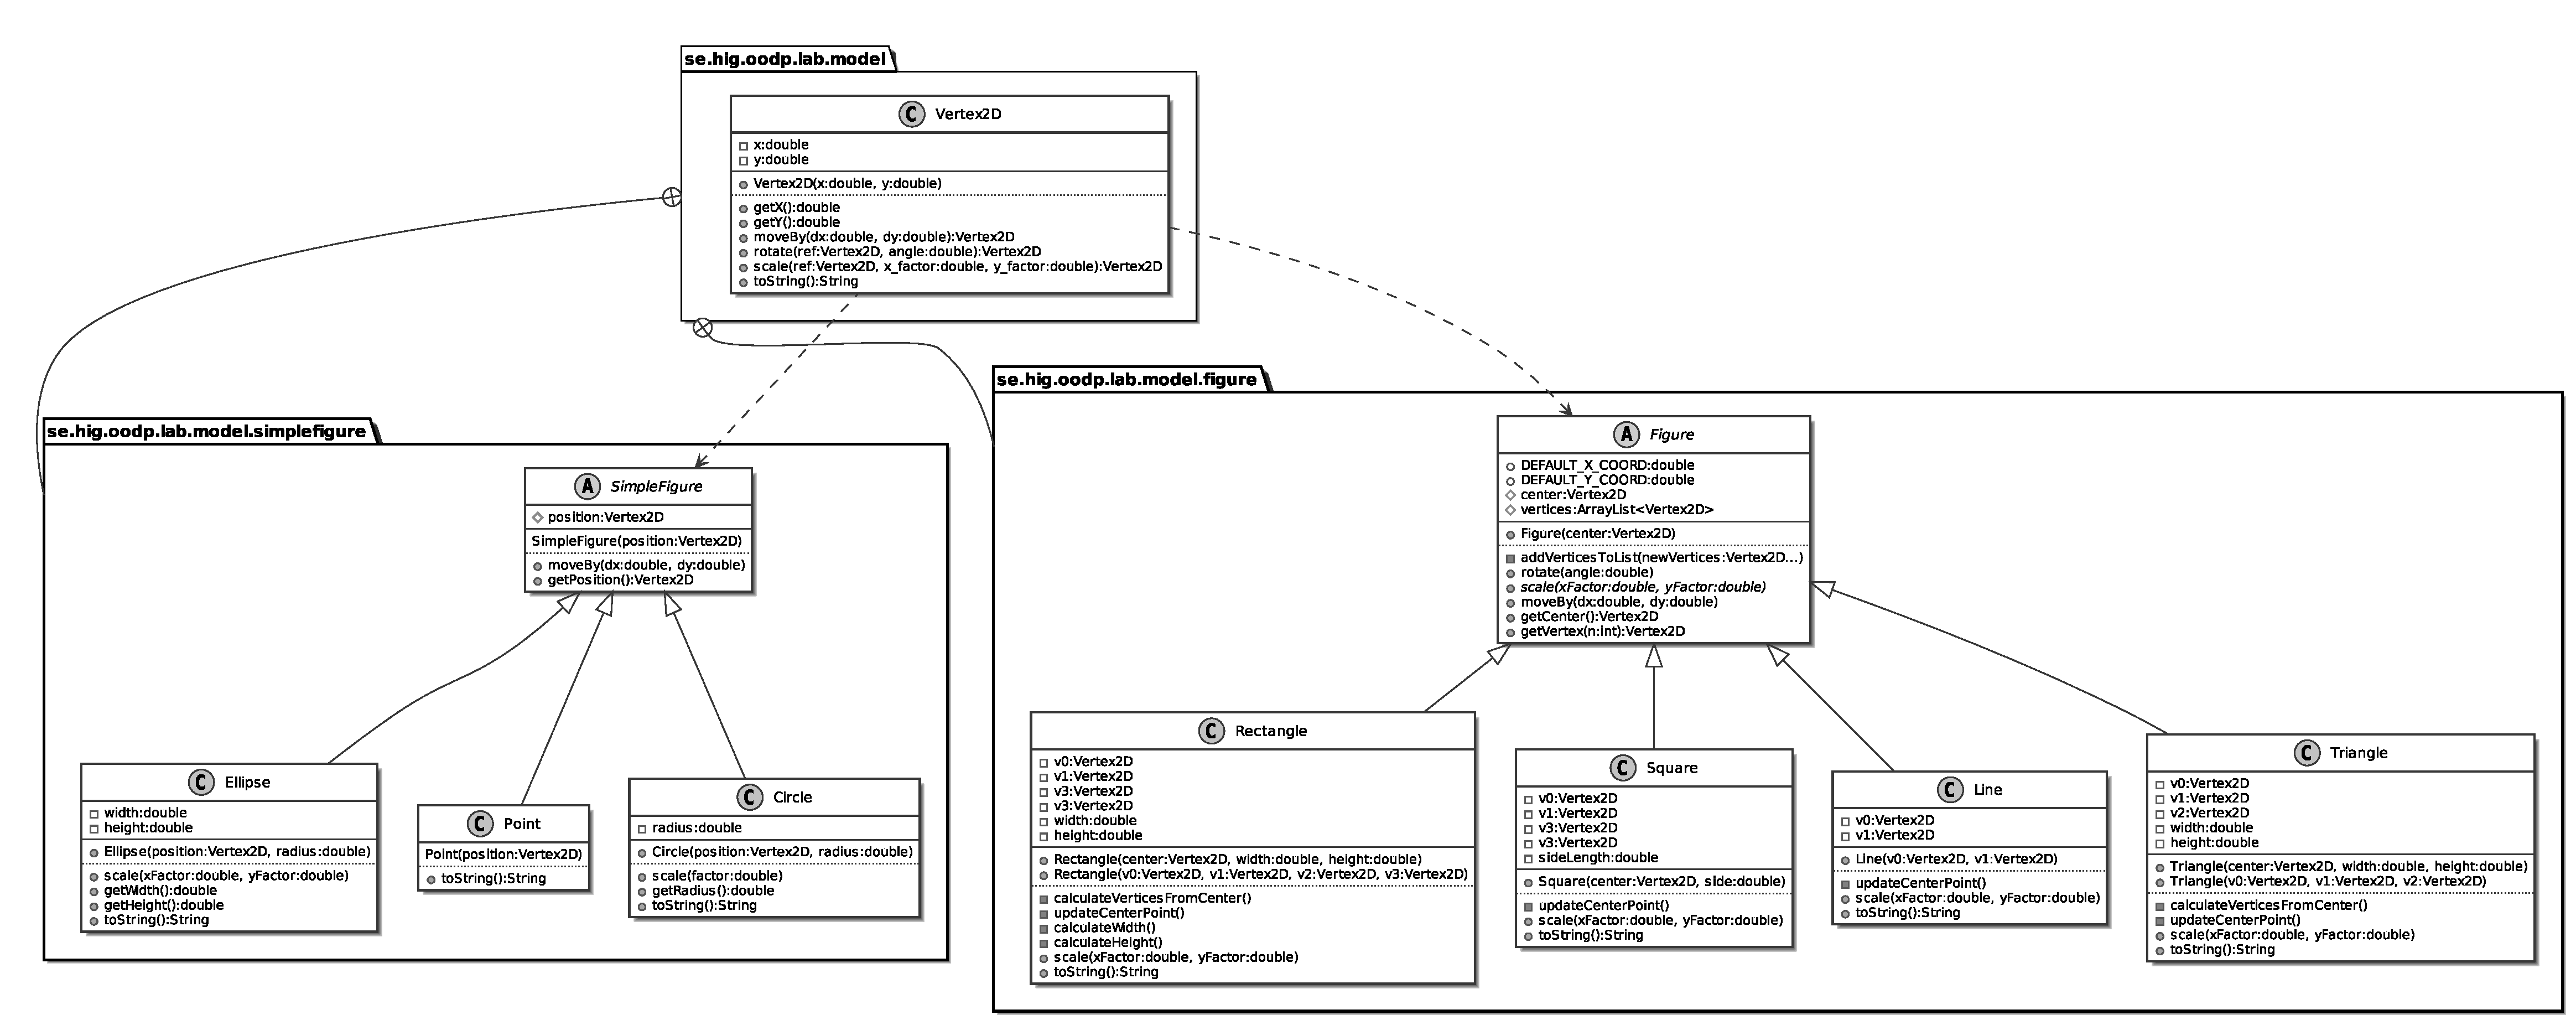
\includegraphics[width=\linewidth]{diagram/uppgift2.eps}
\caption{Uppgift~2\ref{sec:uppg2c}: UML-diagram för geometriska figurer
(\texttt{diagram/uppgift2.eps})}
\label{fig:uppg2a}
\end{sidewaysfigure}


\subsection{}\label{sec:uppg2d}
\subsubsection*{Frågeställning}
Implementera modellen som ni skapade i (c), dvs. aktualisera koden från
uppgift 1 så att den motsvarar klassdiagrammet från (c)!
Använd testen som ni utvecklade i uppgift 1 för att visa att klasserna fungerar
som förut!

\subsubsection*{Lösning}
Se bifogad kod för implementering.
